% !TEX root = thesis_draft.tex

\appendix
\section{Theory of Mind}
\label{app:tom}

A good introduction about Theory of Mind is given by
\textcite[p.~455--467]{postle_essentials_2020}. It defines the key process of
mentalizing as ``engaging in mentation about the thoughts, motivations,
and knowledge of another''. It also lists a number of brain regions associated
with theory of mind: the right posterior temporal sulcus, the temporal poles,
the anterior paracingulate cortex and/or the medial pre-frontal cortex, and
finally (to a lesser degree and with lots of caveats) the temperoparietal
junction. Theory of Mind co-occurs with the development of executive control,
but the mechanism behind that is still an active area of research
\parencite{perner_development_1999,bradford_self_2015}. A high working memory
load will disrupt Theory of Mind ability even in adults
\parencite{maehara_i_2011}, causing them to (incorrectly) fall back on their
own beliefs. Finally, impairments in theory of mind may underlie ASD
\parencite[p.~457]{baron-cohen_does_1985,frith_theory_2005,postle_essentials_2020}.

\section{\citeauthor{newman_effects_2021}'s tacit coordination task}
\label{app:task}

Tacit coordination tasks, i.e. tasks in which participants have to silently work
together, are widely studied: \textcite{de_weerd_higher-order_2015} found
in a simulation study that higher-order theory of mind (`I know that she knows
that I know\ldots') is only useful up to a certain point in such tasks.
\Textcite{de_kwaadsteniet_social-psychological_2012} review different
coordination rules people use in tacit coordination tasks.

To study the effect of working memory on theory of mind,
\textcite{newman_effects_2021} developed a tacit coordination experiment in
which two participants need to look at four images, and pick the same one.
They get to see the other participant's choice after each trial. The
underlying idea is that both participants need to apply theory of mind to
determine how the other participant makes their choice, so both can converge on
a shared strategy and perform at a better than chance level.
\textcite{newman_effects_2021} tested the effect of working memory load on
theory of mind by alternating trials with either a 2-back task
\parencite{kirchner_age_1958} or a 0-back task (i.e. even/odd classification).
During the experiment, EEG data was collected for both participants. That data
is analysed in the current project.

One trial in the experiment consists of a fixation cross screen shown between
1000--3000ms to prevent anticipation effects, a self-paced screen where the
participant sees the images and chooses one and a feedback screen which is shown
for 4000ms. Then, the working memory task takes over with three screens with
the same purpose but different timings: the answering screen in the n-back
task is always shown 3000ms and the feedback screen is shown for only 1500ms.

\begin{figure}[!htpb]
  \includegraphics[width=\linewidth]{../extra/behav/out/summary.pdf}
  \caption{Each dyad's favourite colors for the three parts of the stimulus images.}
  \label{fig:colors}
\end{figure}

Two different abstract stimulus image types are used. One which varies colors,
and one which varies shapes. The stimuli were taken from a game-theoretic
study by \textcite{alberti_salience_2012}. This study focuses on modeling why
participants tend to prefer certain (more `salient') images. Luckily,
\textcite{alberti_salience_2012} found that for the abstract image set the
experiment borrows, these preferences tend not to be structural across
participants (see also Figure~\ref{fig:colors}).

Finally, it is worth mentioning participants in a dyad were matched for gender
and all participants filled in three self-report questionnaires
\parencite{christodoulou_effects_2021}: the Interaction Anxiousness Scale,
the Interpersonal Reactivity Index and the Autism Spectrum Quotient. This
made it possible to check for confounding effects of social anxiety, empathy
and ASD \parencite{akcay_role_2021}.


\section{Linear mixed effect models}
\label{app:lme}

\begin{tabularx}{\linewidth}{| X | X X X |}
\hline
purpose & repetition & base model & extra term\\\hline
effect of window size & by measure & value $\sim$ trial + (1 | session) + (1 | electrode) & winsize\\
effect of taper on PLV & none & plv $\sim$ trial + (1 | session) + (1 | electrode) & taper\\
effect of taper on CCorr & none & ccorr $\sim$ wm\_load + (1 | session) & taper\\
effect of taper on ImagCoh & none & imagcoh $\sim$ trial + (1 | session) + (1 | electrode) & taper\\
effect of resolution on PLV & none & plv $\sim$ trial + wm\_load + (1 | session) + (1 | electrode) & resolution\\
effect of resolution on CCorr & none & ccorr $\sim$ wm\_load + (1 | session) + (1 | electrode) & resolution\\
effect of resolution on ImagCoh & none & imagcoh $\sim$ trial + stim\_type + (1 | session) + (1 | electrode) & resolution\\
effect of trial & by measure, electrode, band & value $\sim$ 1 + (1 | session) & trial\\\hline
\end{tabularx}

Note that the random effect structure of the final model is not always supported
by the data, but we decided it better to sometimes have a `singular fit' error
than to have a model that sometimes does not account for the structure within
sessions.


\section{Supplementary figures}
\label{app:supplementaryfigures}

\begin{figure}[!htpb]
  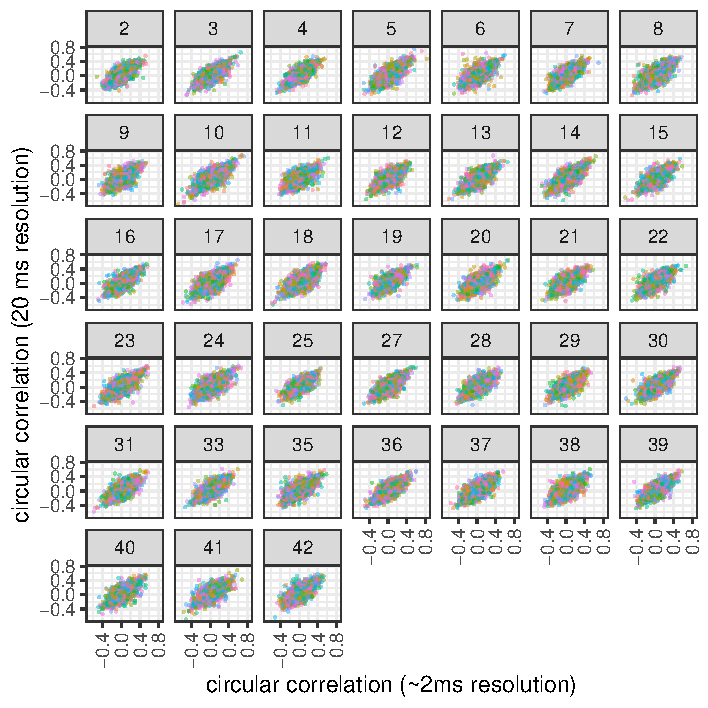
\includegraphics[width=\linewidth]{../stats/results/resolutionapp.png}
  \caption{Circular correlation values do not correlate perfectly across different frequency analysis resolutions, contrary to phase locking values and imaginary part of coherency values (not shown here). Each subplot represents a single session. Each dot represents the data for a single timepoint. Colours are assigned based on electrode.}
  \label{fig:resolutionapp}
\end{figure}

\begin{figure}[!htpb]
  \includegraphics[width=\linewidth]{../stats/results/imagcoh-theta.pdf}
  \caption{Predicted imaginary part of coherency without random effects in the theta band.}
  \label{fig:imagcohtheta}
\end{figure}

\begin{figure}[!htpb]
  \includegraphics[width=\linewidth]{../stats/results/slopes_theta.pdf}
  \caption{One inter-brain synhrony value is calculated per trial in the theta band. (A) shows their (average) slope when we fit a line through them. (B) shows none of these slopes are significantly different from zero after FDR correction by comparing a linear mixed effect model that includes the slope to one that does not for each electrode.}
  \label{fig:slopes_theta}
\end{figure}

\begin{figure}[!htpb]
  \includegraphics[width=\linewidth]{../stats/results/learning_curve_logistic.pdf}
  \caption{Logistic regression: performance on the train and test set during cross-validation for different regularization parameters. The triangle shows the parameter used for final evaluation.}
  \label{fig:learning_curve_logistic}
\end{figure}

\begin{figure}[!htpb]
  \includegraphics[width=\linewidth]{../stats/results/learning_curve_svm.pdf}
  \caption{SVM: performance on the test set during cross-validation for different regularization and radial basis function size parameters. The triangle shows the parameters used for final evaluation.}
  \label{fig:learning_curve_svm}
\end{figure}

\begin{figure}[!htpb]
  \includegraphics[width=\linewidth]{../stats/results/learning_curve_rf.pdf}
  \caption{Random Forest: performance on the test set during cross-validation for different number of estimators and maximum amounts of features. The triangle shows the parameters used for final evaluation.}
  \label{fig:learning_curve_rf}
\end{figure}

\begin{figure}[!htpb]
  \includegraphics[width=\linewidth]{../stats/results/learning_curve_mlp.pdf}
  \caption{Multi-layer perceptron: performance on the test set during cross-validation for different learning rates. The triangle shows the rate used for final evaluation.}
  \label{fig:learning_curve_mlp}
\end{figure}

\begin{figure}[!htpb]
  \includegraphics[angle=90,width=.95\linewidth]{../stats/results/learning_curve_within_dyad.pdf}
  \caption{Within-dyad SVM classifiers: performance on the test set during cross-validation for different regularization and SVM RBF gamma parameters. A triangle shows the parameters used for final evaluation. One plot for each session and WM manipulation.}
  \label{fig:learning_curve_within_dyad}
\end{figure}
